
%   i.) Describe all the steps of a Deep Learning FL system
%      
%

%how do FL systems work in general?
Feature location systems retrieve a ranked list of program elements
(e.g. methods, classes) for a developer query. In the {\em indexing}
phase, feature location systems commonly construct a model of the
software, at the granularity of program elements, based on the natural
language embedded in identifiers and comments. In the {\em retrieval}
phase, given a natural language query, feature location systems use
the model to retrieve all of the relevant program elements with high
similarity to the query.

\subsection{Feature Location Workflow}

%how does a deep learning system differ
A feature location system based on deep learning, during its indexing
phase, creates a contextual representation of the natural language
terms embedded in the source code. This contextual representation
includes influence from terms preceding and following each term,
relative to their distance from that term. More intuitively, such
models incoporate mutual influence between terms in the same method,
while terms that are closer in distance (e.g. occur the same
statement) influence each other more strongly. 



\begin{figure}[tb]
\centering
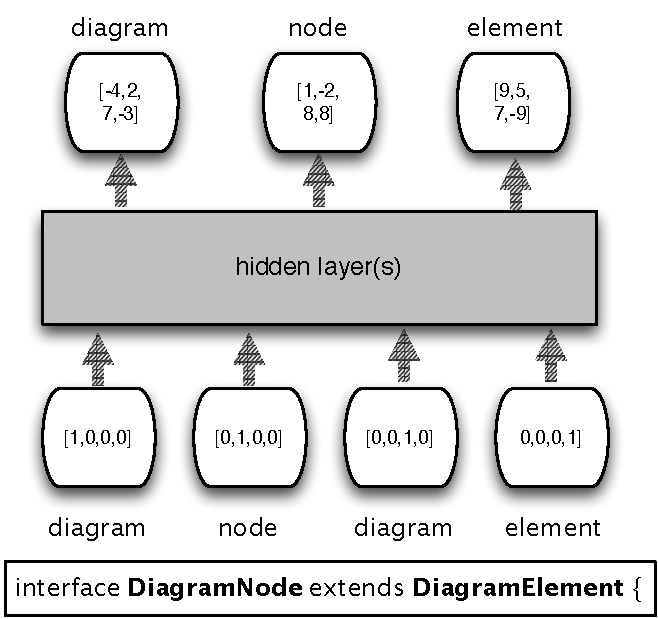
\includegraphics[width=.9\columnwidth]{figures/neuralnet.pdf}
\caption{A deep learning neural network encodes source code identifiers,
in the order they apprear in the source code, in its input
layer. Using a deep structure of hidden layers, each term and its
context recieves a semantic vector representation.}
\label{figure:miningworkflow}
\end{figure}



%what is deep learning
Deep learning is based on a multi-stage neural network, consisting of
several hidden layers in addition to single input and output layers.
The input layer consists of the ordered sequences of identifiers
extracted from the code. The multiple hidden layers serve to capture
the context for each encountered term, representing the complex
patterns of term contexts occuring in the corpus. The output layer
consists of a vector for each term, which has been shown to carry
semantic meaning. Recent advances in this area have stemmed from the
use of novel neural network architectures, including recurrent neural
networks that connect the hidden layers back to the input layer, among
other strategies. The systems are trained using backpropagation and
gradient descent, techniques common to many neural network based
models.

 
%preprocessing
A number of preprocessing steps are commonly performed during the
indexing phase of feature location systems including word stemming,
which reduces terms to their base form (e.g. running $\rightarrow$
run), and stop word removal, which removes common words (e.g. the, is,
at). Additional preprocessing steps are required for source code, such
as identifier splitting, ensuring that composite identifiers are
divided into their constituent terms (e.g. addToCart $\rightarrow$
add,to,cart). 


During the retrieval state of feature location, a similarity measure
(e.g. cosine similarity) between the words in the query and words in
each program element is computed. The program elements are ranked
based on this similarity metric and presented to the developer in
descending order.



%Chris: I assume this is what gensim is doing, but I am not sure...




\subsection{Semantic Similarity}
